\documentclass[15pt,a5paper,reqno]{article}
\usepackage{hyperref}
\usepackage[warn]{mathtext}
\usepackage[utf8x]{inputenc}
\usepackage{amssymb, amsmath, multicol}
\usepackage[russian]{babel}
\usepackage{graphicx}
\usepackage[shortcuts,cyremdash]{extdash}
\usepackage{wrapfig}
\usepackage{floatflt}
\usepackage{lipsum}
\usepackage{verbatim}
\usepackage{concmath}
\usepackage{euler}
\usepackage{xcolor}
\usepackage{etoolbox}
\usepackage{fancyhdr}
\usepackage{subfiles}
\usepackage{enumitem}
\usepackage{amsthm}
\usepackage{indentfirst}
\usepackage{import}

\DeclareMathOperator{\sign}{sign}

\RequirePackage[ left     = 1.5cm,
  right    = 1.5cm,
  top      = 2.0cm,
  bottom   = 1.25cm,
  includefoot,
  footskip = 1.25cm ]{geometry}
\setlength    {\parskip}        { .5em plus .15em minus .08em }
%\setlength    {\parindent}      { .0em }
\renewcommand {\baselinestretch}{ 1.07 }

\fancyhf{}

\renewcommand{\footrulewidth}{ .0em }
\fancyfoot[C]{\texttt{\textemdash~\thepage~\textemdash}}
\fancyhead[R]{\hfilШурыгин}

\makeatletter
\patchcmd\l@section{%
  \nobreak\hfil\nobreak
}{%
  \nobreak
  \leaders\hbox{%
    $\m@th \mkern \@dotsep mu\hbox{.}\mkern \@dotsep mu$%
  }%
  \hfill
  \nobreak
}{}{\errmessage{\noexpand\l@section could not be patched}}
\makeatother
\parindent = 1cm % отступ при красной строке⏎
\pagestyle{fancy}    
\renewcommand\qedsymbol{$\blacksquare$}

\newcommand{\when}[2]{
  \left. #1 \right|_{#2} \hspace
}
\renewcommand{\kappa}{\varkappa}
\RequirePackage{caption2}
\renewcommand\captionlabeldelim{}
\newcommand*{\hm}[1]{#1\nobreak\discretionary{}

\DeclareSymbolFont{T2Aletters}{T2A}{cmr}{m}{it}
{\hbox{$\mathsurround=0pt #1$}}{}}
% Цвета для гиперссылок
\definecolor{linkcolor}{HTML}{000000} % цвет ссылок
\definecolor{urlcolor}{HTML}{799B03} % цвет гиперссылок
 
\hypersetup{pdfstartview=FitH,  linkcolor=linkcolor,urlcolor=urlcolor, colorlinks=true}


%\setcounter{secnum[utf8x]depth}{0}

\begin{document}

% НАЧАЛО ТИТУЛЬНОГО ЛИСТА
\begin{center}
  {\small ФЕДЕРАЛЬНОЕ ГОСУДАРСТВЕННОЕ АВТОНОМНОЕ ОБРАЗОВАТЕЛЬНОЕ\\ УЧРЕЖДЕНИЕ ВЫСШЕГО ОБРАЗОВАНИЯ\\ МОСКОВСКИЙ ФИЗИКО-ТЕХНИЧЕСКИЙ ИНСТИТУТ\\ (НАЦИОНАЛЬНЫЙ ИССЛЕДОВАТЕЛЬСКИЙ УНИВЕРСИТЕТ)\\ ФИЗТЕХ-ШКОЛА РАДИОТЕХНИКИ И КИБЕРНЕТИКИ}\\
  \hfill \break
  \hfill \break
  \hfill \break
  \Huge{Дифракция света на периодических структурах (саморепродукция).}\\
\end{center}

\hfill \break
\hfill \break
\hfill \break
\hfill \break
\hfill \break
\hfill \break

\begin{flushright}
  \normalsize{Работу выполнил:}\\
  \normalsize{\textbf{Шурыгин Антон Алексеевич, группа Б01-909}}\\
\end{flushright}

\begin{center}
  \normalsize{\textbf{Долгопрудный, 2021}}
\end{center}


\thispagestyle{empty} % выключаем отображение номера для этой страницы

% КОНЕЦ ТИТУЛЬНОГО ЛИСТА

\newpage
\thispagestyle{plain}
\tableofcontents
\thispagestyle{plain}
\newpage


\textbf{Цель работы:}
Изучение явления саморепродукции и применение его к измерению параметров периодических структур.

\textbf{Оборудование:} лазер,кассета с сетками, мира, короткофокусная линза с микрометрическим винтом, экран, линейка.

\section{Введение и краткая теория}
При дифракции на предмете с периодической структурой наблюдается явление саморепродукции: на некотором расстоянии от предмета вдоль направления распространения волны появляется изображение, которое потом периодически повторяется.  \par
Представим волну за периодическим объектом в виде суммы плоских волн разных направлений. Отдельные слагаемые плоские волны называют пространственными гармониками. Вдоль пути распространения волнового фронта на некотором расстоянии $z_0$ от предмета существует плоскость, где разность фазовых набегов любых пространственных гармоник (плоских волн идущих под углом $\theta$т к оси распространения), входящих в состав суперпозиции, кратна $2T$ В этой плоскости фазовые соотношения между всеми плоскими волнами, входящими в состав суперпозиции, такие же, что и в предметной плоскости. Поэтому в результате интерференции этих волн возникает изображение, тождественное исходному периодическому объекту. Все сказанное справедливо для любого расстояния $z_n$, кратного $z_0$. Для решетки с периодом $d$.
\begin{equation}
    z_n = \frac{2d^2}{\lambda}n
\end{equation}

Суть эксперимента по саморепродукции состоит в том, что дифрагированная на периодическом транспаранте (решетка, сетка) плоская монохроматическая волна лазера (лазерный пучок) воспроизводит изображение транспаранта без каких-либо оптических элементов.

\begin{figure}[h!]
    \centering
    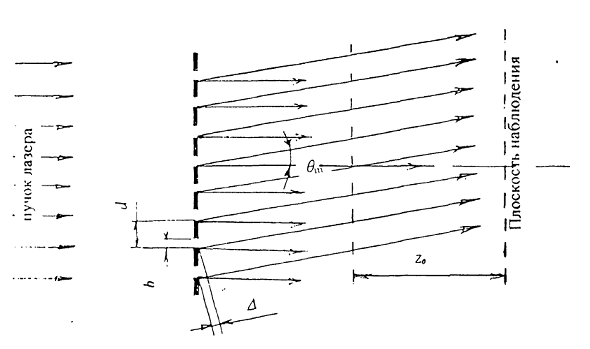
\includegraphics[width=15cm]{pics/fig1.png}
    \caption{Дифракция лучей на сетке и возникновение саморепродуцированного изображения}
    \label{fig:vac}
\end{figure}

\section{Схема установки}

\begin{figure}[h!]
    \centering
    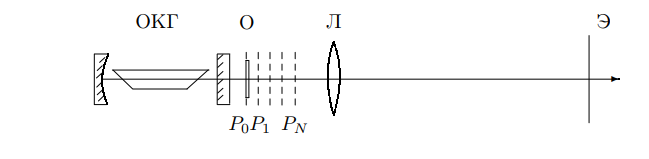
\includegraphics[width=15cm]{pics/scheme.png}
    \caption{Схема лабораторной установки}
    \label{fig:vac}
\end{figure}

\section{Ход работы}


\subsection{Измерение периода решеток по их пространственному спектру}


\begin{table}[h!]
	\centering
	\begin{tabular}{| c | c | c | c | c | c |}
    \hline
    $n_{сетки}$ & $X_m$, мм & $m$ & $x$, мм  & $d$, мм & $\sigma_d$, мм\\
    \hline
    1 & 201  & 6 & 33.50  &  0.020 & <0.001\\
    \hline
    2 & 223 & 9 & 24.77  &   0.027 & <0.001\\
    \hline
    3 & 177  & 16 & 11.1 &   0.061 & 0.001\\
    \hline
    4 & 235  & 24 & 9.79   &  0.069 & 0.001\\
    \hline
    5 & 63  & 16 & 3.93    &   0.174  & 0.007\\
    \hline
    \end{tabular}
    
	\caption{Измерение расстояние между соседними дифр. макс. на экране}
	\label{nu1}
\end{table}


Расстояние от кассеты до экрана $L = 124 \: cm$, $\lambda = 560 \: nm$.

\begin{equation}
    dsin(\theta_x) = m_x \lambda, \:\:\:\: d sin(\theta_y) = m_y \lambda     
  \label{first}
\end{equation}

Полагая $sin(\theta) \backsimeq \theta \backsimeq \frac{x}{L}$, найдем с помощью формул (1) период каждой решетки.

\[     d = \frac{\lambda L}{x}        \]

Измерения и результаты вычисления периоды дифракционной решетки занесены в таблицу 1.



\subsection{Измерение периода решеток по изображению, увеличенного с помощью линзы}

Найдем период решетки другим способом.
 
\begin{table}[h!]
	\centering
	\begin{tabular}{| c | c | c | c | c |}
\hline
$n_сетки$ & $x_m, mm$ & $m$ & $D, mm$ & $d, mm$\\
\hline
1 & - & - & - & -\\
\hline
2 & 3,5 & 6 & 0,58 & 0,027 \\
\hline
3 & 9 & 6 & 1,5 & 0,072\\
\hline
4 & 12 & 4 & 3 & 0,144\\
\hline
5 & 16 & 4 & 4 &  0,192\\
\hline
\end{tabular}

	\caption{Определение размера клеток $D$}
	\label{nu1}
\end{table}


Измеренные расстояния: между сеткой и экраном - $a' = 131 \: cm \rightarrow$ между линзой и сеткой -  $a = a' - b = 6 \: cm$ , между линзой и экраном - $ b= 125\:cm$.

\[    d = \frac{a}{b} \cdot D   \]

Таким образом по формуле выше находим период решетки и записываем результат в таблицу 2. 


\subsection{Исследование саморепродукции с помощью сеток}

Исследуем саморепродукцию.
Находим координаты $z_n$ плоскостей саморепродукции, строим график. По коэффициенту наклона прямой графика определим период решетки по формуле:

\begin{equation}
  d_i = \sqrt{\frac{k_i\lambda}{2}}
\end{equation}


\begin{table}[h!]
	\centering
	\begin{tabular}{| c | c | c | c | c | c |}
    \hline
          & $z_3, mm$ & $z_4, mm$  & $z_5, mm$\\
    \hline
        1 & - & 4 & 8,1 & 6,4 & 21,5\\
    \hline
        2 & - & 8,55 & 15,1 & 22,1 & 43,5\\
    \hline
        3 & - & 12,2 & 22 & 33,2 & 65,5\\
    \hline
        4 & - & 17,55 & 28,5 & 49,2 & -\\
    \hline
        5 & - & 20,55 & 35,2 & 59,7 & -\\
    \hline
        6 & - & 23,6 & 42 & - & -\\
    \hline
        7 & - & 28,8 & 49 & - & -\\
    \hline
        8 & - & - & 55,5 & - & -\\
  \hline
  \end{tabular}

	\caption{Измерение номера дифракционной картины от координаты линзы}
	\label{nu1}
\end{table}

\begin{table}[h!]
	\centering
	\begin{tabular}{| c | c | c | c | c | c |}
    \hline
    $n_сетки$ & 1 & 2 & 3 & 4 & 5  \\
    \hline
    $d, mm$   & - & 0,034 & 0,043 & 0,061 & 0,077   \\
    \hline
\end{tabular}
	\caption{Резульаты вычисления периода дифракционных решеток}
	\label{nu1}
\end{table}

Измерения и полученные значения сводим в таблицу 3. 
Затем строим графики $z = f(n)$.


\begin{figure}[h!]
  \centering
  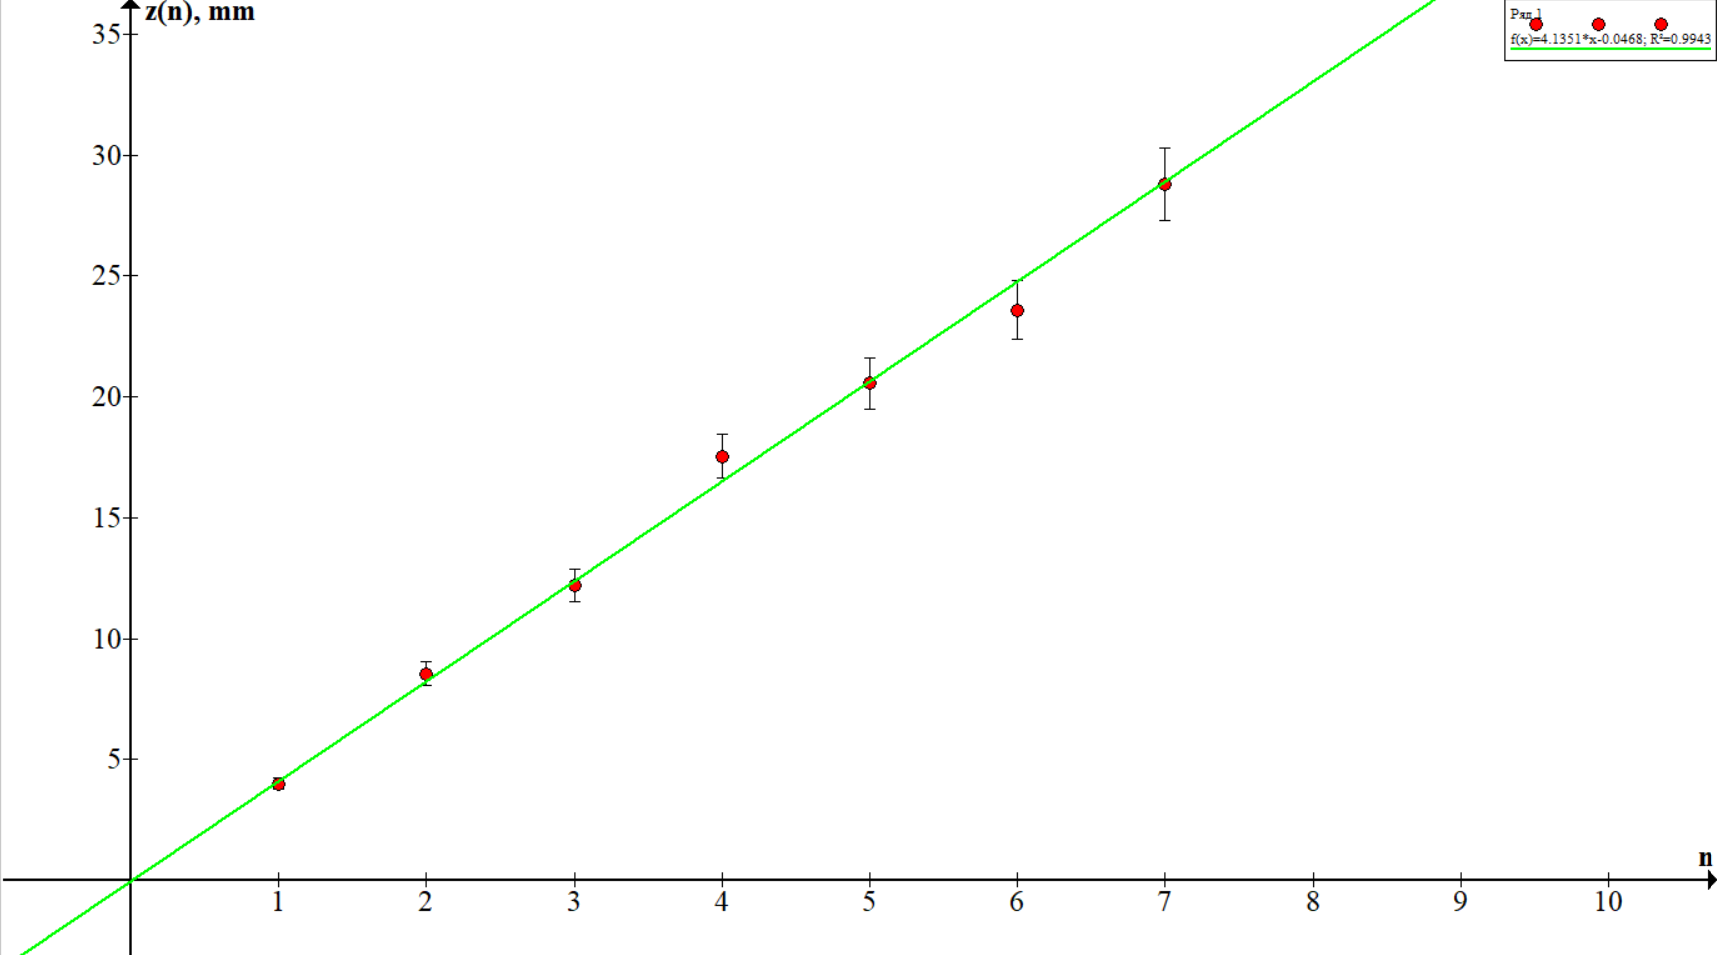
\includegraphics[width=13cm]{pics/lab_436_1.png}
  \caption{График $z_1 = f(n)$}
  \label{}
\end{figure}

\begin{figure}[h!]
  \centering
  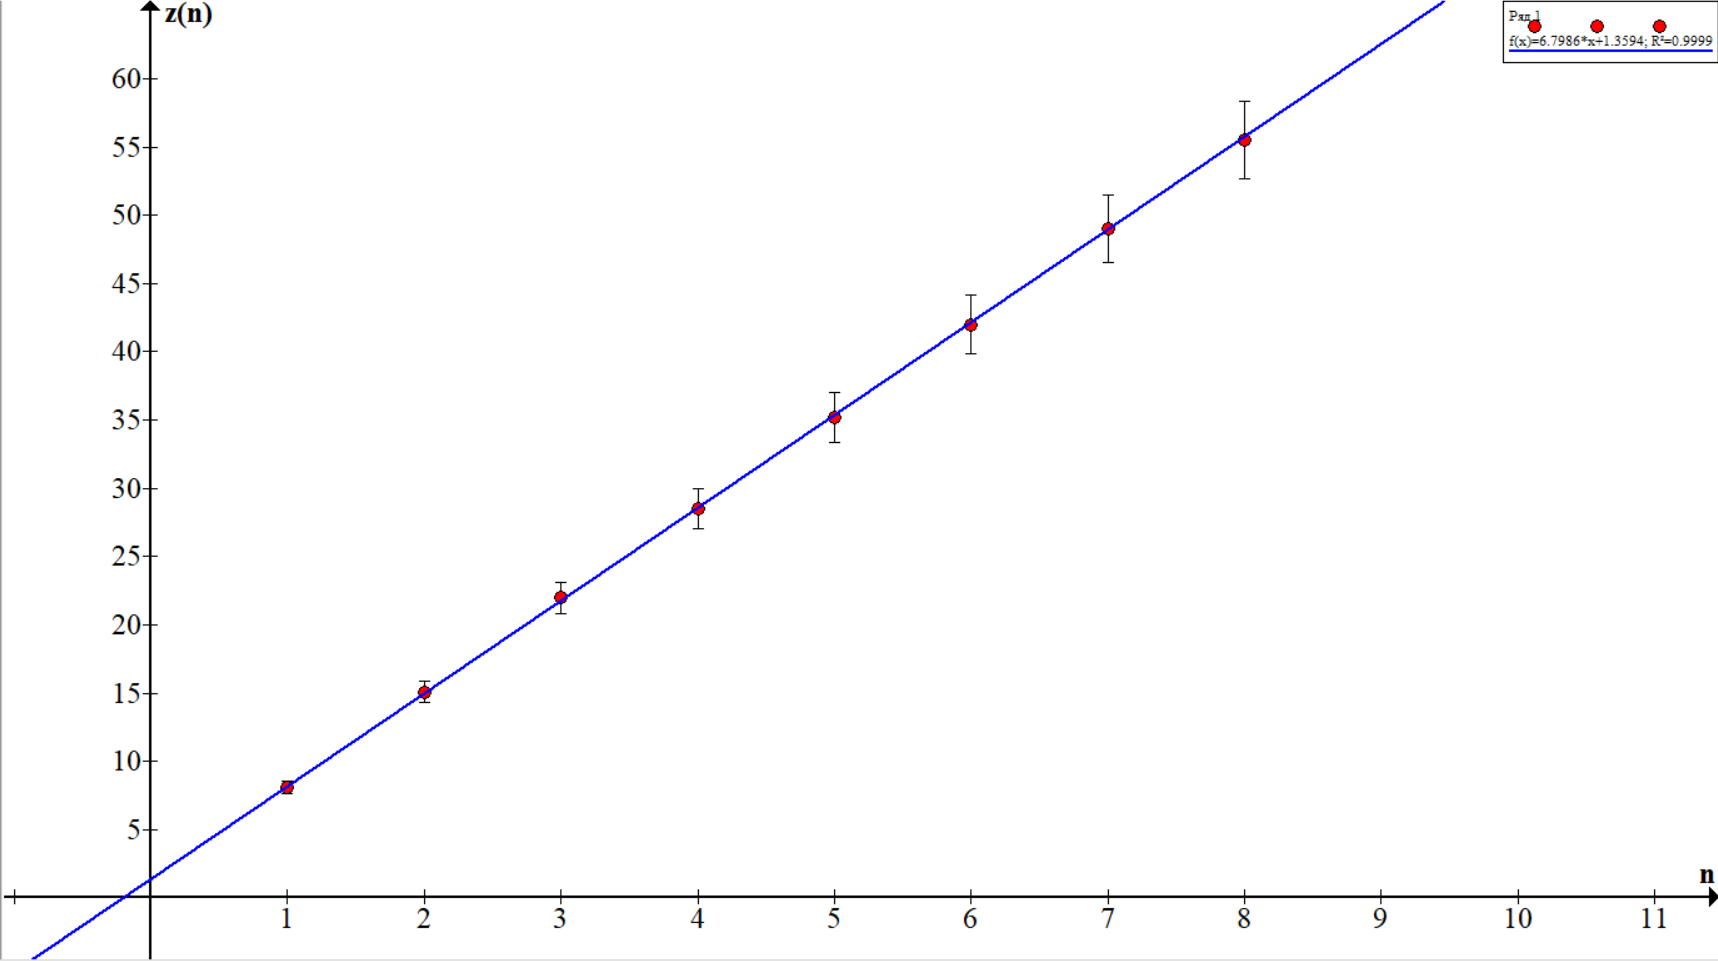
\includegraphics[width=13cm]{pics/lab_436_2.png}
  \caption{График $z_2 = f(n)$}
  \label{}
\end{figure}


\begin{figure}[h!]
  \centering
  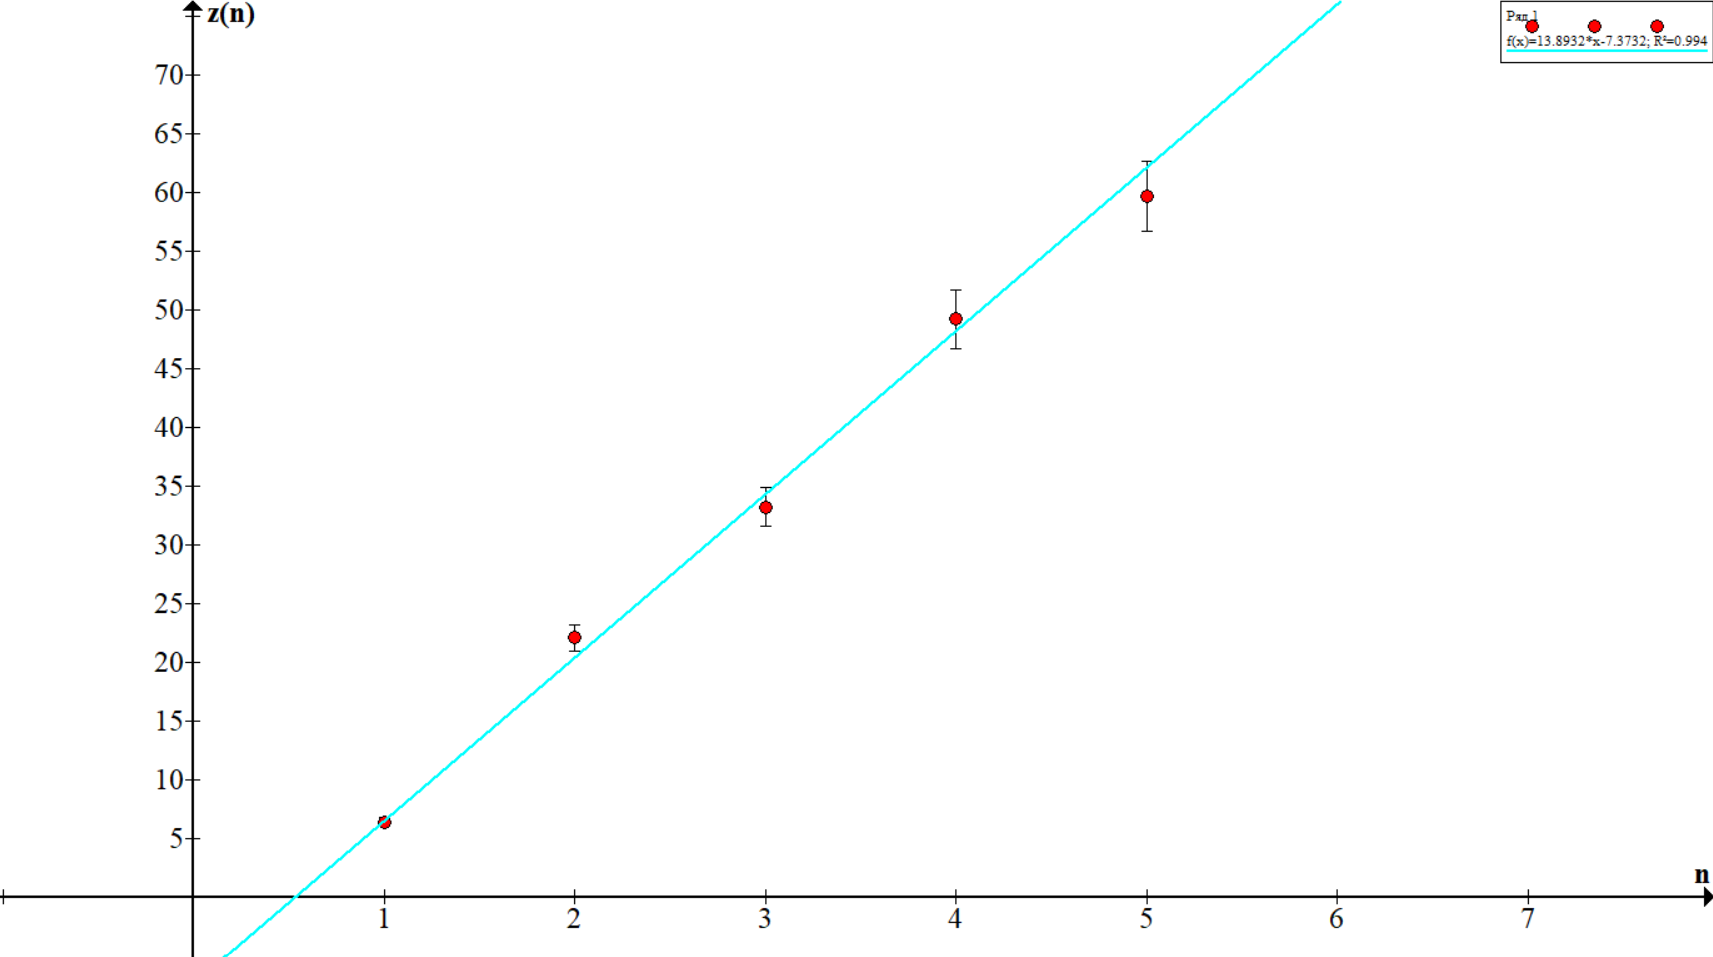
\includegraphics[width=13cm]{pics/lab_436_3.png}
  \caption{График $z_3 = f(n)$}
  \label{}
\end{figure}


\begin{figure}[h!]
  \centering
  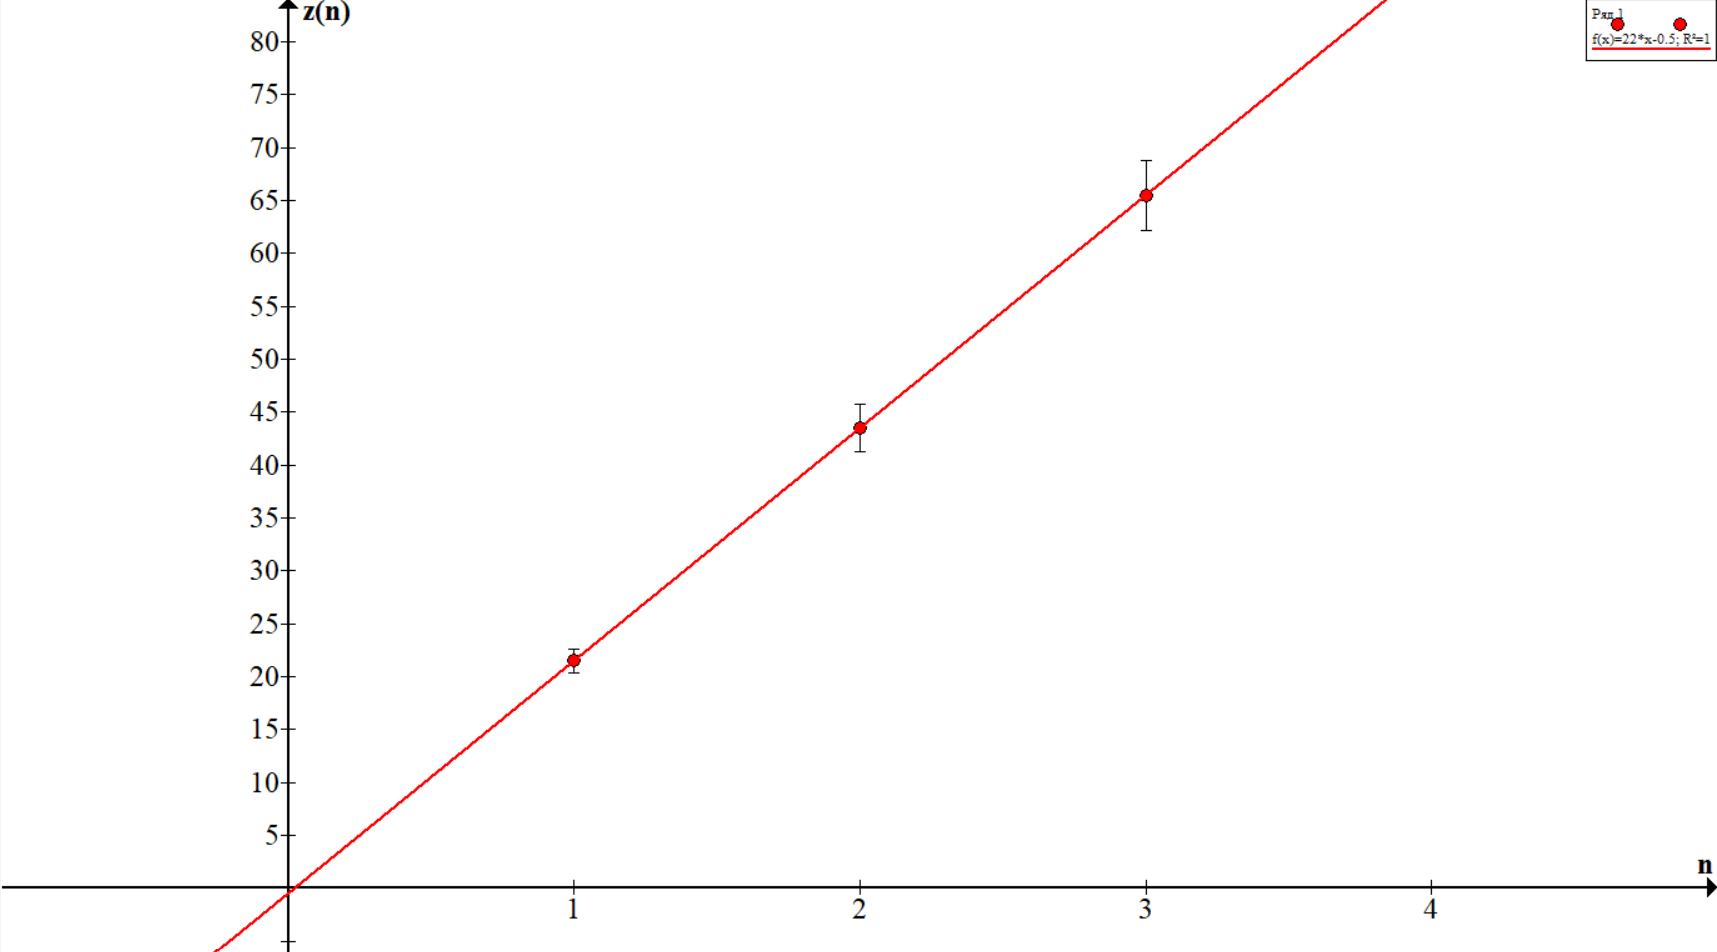
\includegraphics[width=13cm]{pics/lab_436_4.png}
  \caption{График $z_4 = f(n)$}
  \label{}
\end{figure}


\subsection{Исследование миры}

Измеряем расстояние между экраном и линзой - $L_3$, экраном и мирой - $L_4$.
Получаем, что $L_3 = 126 cm$, $L_4 = 132 cm$.

Ширина штриха миры равна $1 mm$.




\begin{table}[h!]
	\centering
	\begin{tabular}{| c | c | c |}
\hline
$n$ & $z_n (25), mm$ & $z_n (20), mm$\\
\hline
-3 & 17 & 12,2\\
\hline
-2 & 20 & 17,2\\
\hline
-1 & 23 & 22,5\\
\hline
0 & 26,1 & 28\\
\hline
1 & 28,3 & 33\\
\hline
2 & 31,9 & 38\\
\hline
3 & 34,5 & 43,5\\
\hline
4 & 37,5 & 48,5\\
\hline
5 & 41,1 & -\\
\hline
\end{tabular}

	\caption{Исследование решеток миры}
	\label{nu1}
\end{table}

\end{document}